% !TEX root = main.tex

\section{Венгерский метод решения задачи о назначениях}

Данный метод применяется для решения задачи о назначениях в форме задачи минимизации. 
Если матрица C интерпретируется как матрица прибыли, задача о назначениях принимает 
форму задачи максимизации. Для сведения данной задачи к задаче минимизации необходимо 
преобразовать матрицу C.

\section{Схема алгоритма Венгерского метода}

\begin{figure}[h!]
    \begin{center}
        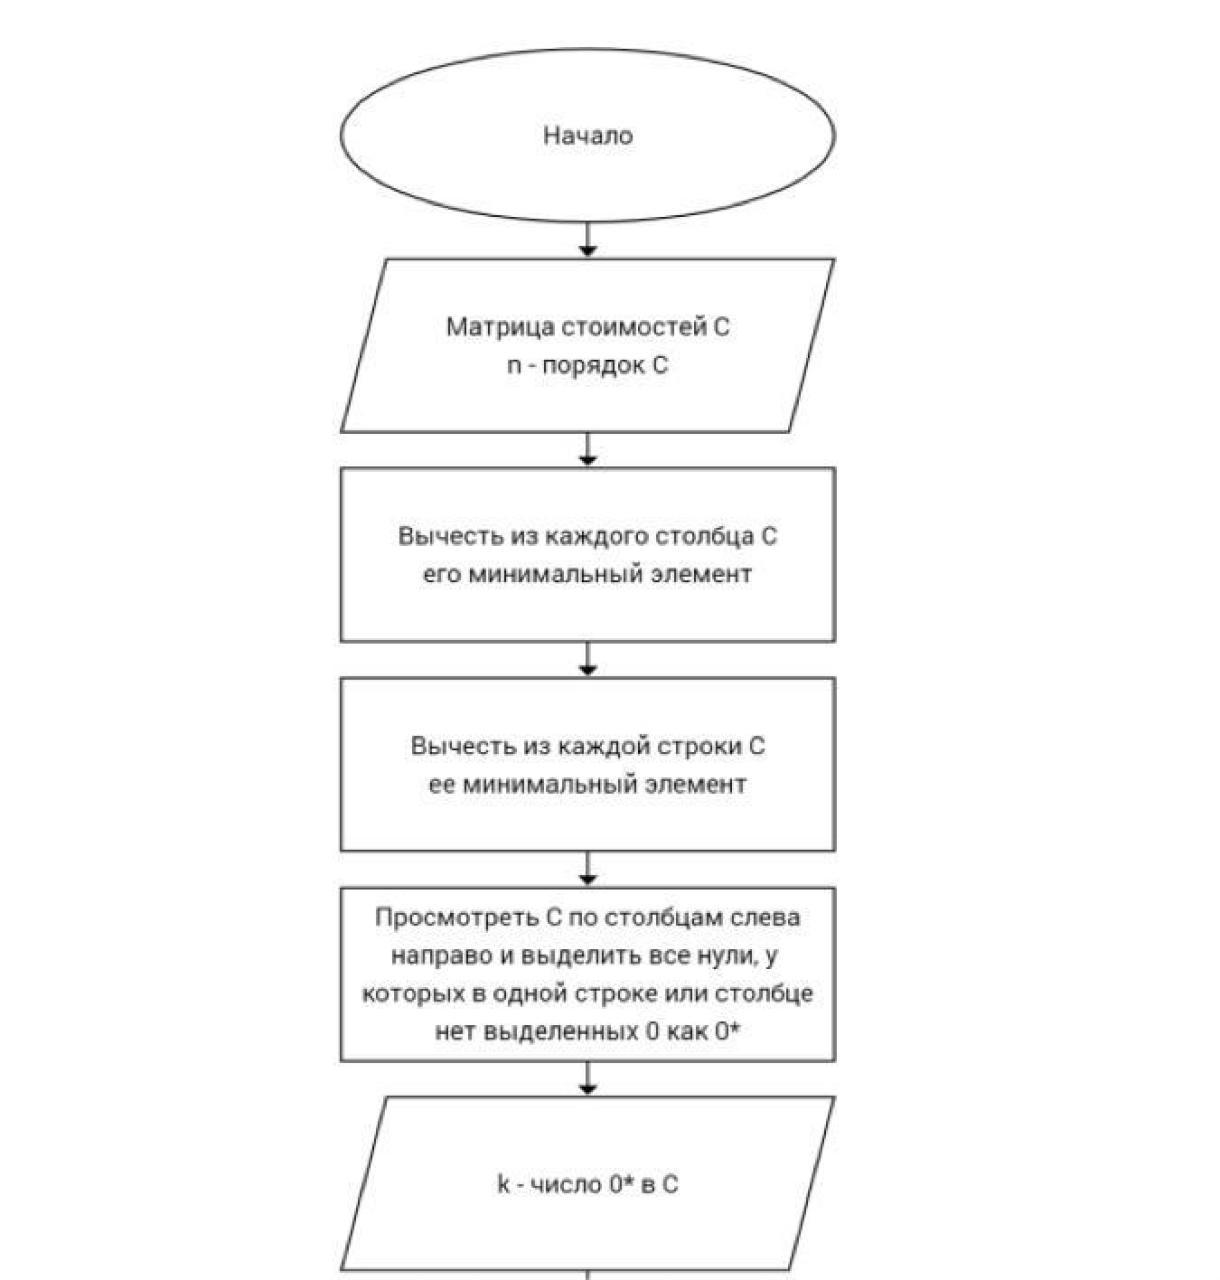
\includegraphics[width=\textwidth]{title/prepare.jpg}
    \end{center}
\end{figure}

\begin{figure}[h!]
    \begin{center}
        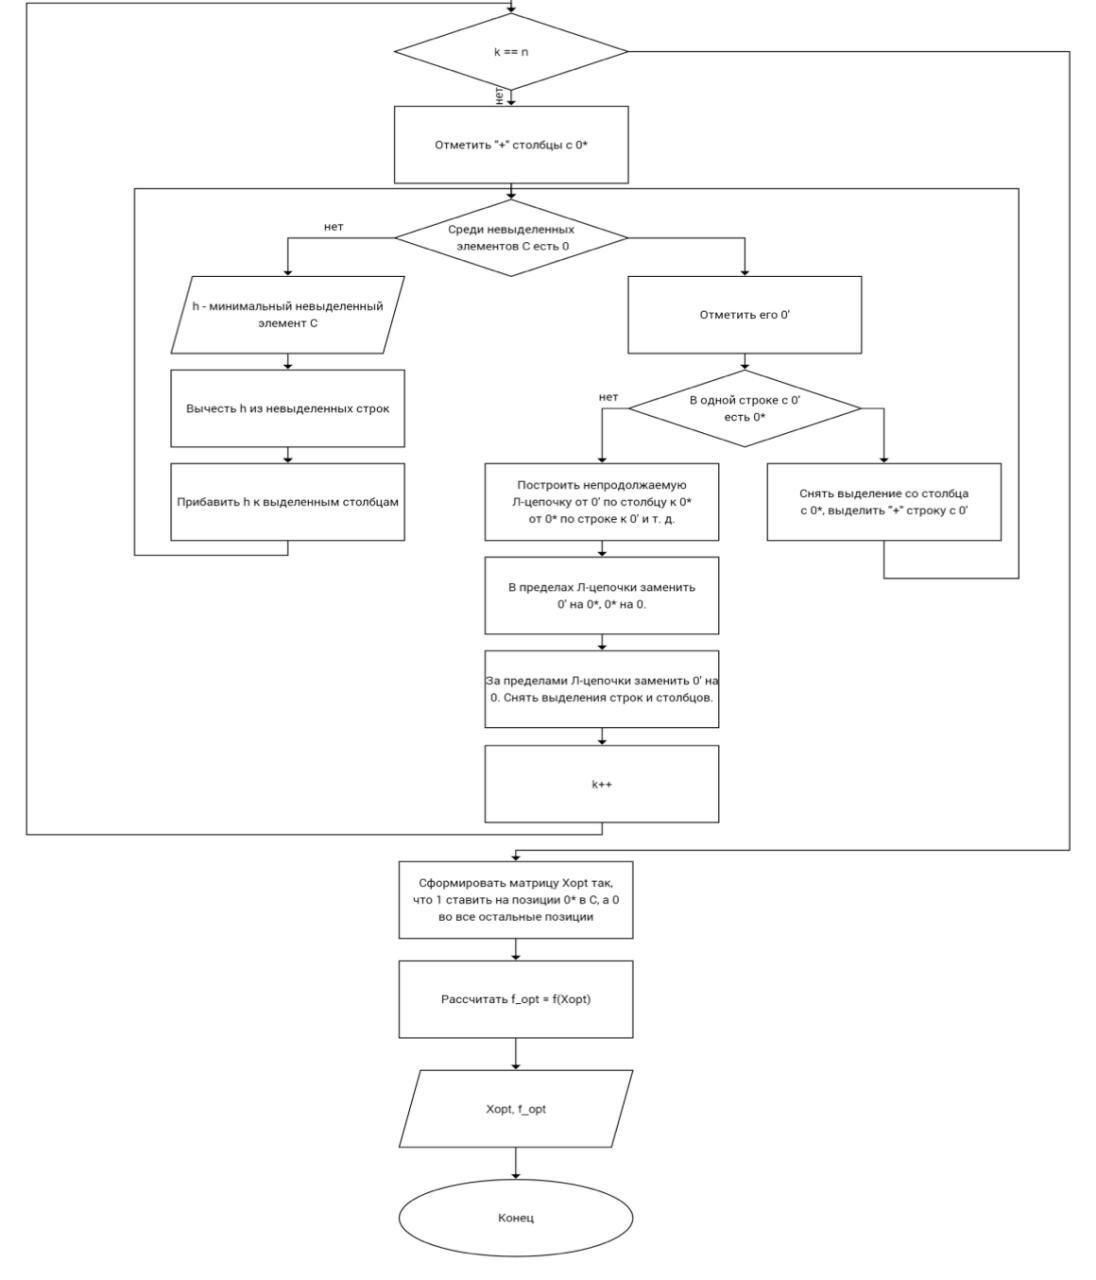
\includegraphics[width=\linewidth]{title/main.jpg}
    \end{center}
\end{figure}